\documentclass[a4paper]{ifacconf}

\usepackage{graphicx,amsmath,url} 
\usepackage[round]{natbib}        
\usepackage[brazil,english]{babel}
\usepackage[T1]{fontenc}
\usepackage[utf8]{inputenc}
\usepackage{ae}
\usepackage{esdiff}

\graphicspath{{../common/figures/}}
\raggedbottom

\newtheorem{teorema}[thm]{{\em Teorema}}{ }
\newtheorem{lema}[thm]{{\em Lema}}{ }
\newtheorem{corolario}[thm]{{\em Corolário}}{ }
\newenvironment{prova}{{\bf Prova.}}{ }

\begin{document}

\selectlanguage{brazil}

\begin{frontmatter}
  \title{Embarque de Rede Neural Recorrente Fenomenologicamente Informada como Analisador Virtual para Sistemas Dinâmicos}

  \author[poliufba]{Silas Henrique Alves Araújo}
  \author[poliufba]{Leonardo Silva de Souza}
  \author[poliufba]{Raony Maia Fontes}
  \author[poliufba]{Márcio André Fernandes Martins}

  \address[poliufba]{Escola Politécnica, Universidade Federal da Bahia, BA, (e-mail: silasaraujo@ufba.br, lssouza@ufba.br, raony@ufba.br, marciomartins@ufba.br)}


  \selectlanguage{english}
  \renewcommand{\abstractname}{{\bf Abstract:~}}
  \begin{abstract}
    The use of Physics-Informed Recurrent Neural Networks (PIRNNs) offers a promising framework for modeling dynamic systems. They combine traditional machine learning with the system's phenomenological model by incorporating differential equations directly into the cost function.
    This work presents the deployment of a PIRNN on a low-cost microcontroller to operate as a virtual analyzer, tested in a software-in-the-loop environment for a system of cascading spherical tanks.
    The results demonstrate reductions of over three times in computation time and the ability to provide information in the absence of measurements. These findings suggest that PIRNNs can be an efficient solution for systems requiring real-time control and process analysis applications.

    \vskip 1mm
    \selectlanguage{brazil}
    {\noindent \bf Resumo}:  O uso de Redes Neurais Recorrentes Fenomenologicamente Informadas (PIRNNs) tem se mostrado promissor na modelagem de sistemas dinâmicos. Elas combinam o aprendizado de máquina tradicional com o modelo fenomenológico do sistema incorporando equações diferenciais diretamente na função de custo.
    Este trabalho apresenta o embarque de uma PIRNN em um microcontrolador de baixo custo para operar como analisador virtual, testado em ambiente \textit{software-in-the-loop} para um sistema de tanques esféricos em cascata.
    Os resultados demonstram reduções superiores a três vezes no tempo de cômputo e a capacidade de fornecer informações na ausência de medições. Esses achados sugerem que a PIRNN pode ser uma solução eficiente para sistemas que exigem controle em tempo real e aplicações de análise de processos.
  \end{abstract}

  \selectlanguage{english}

  \begin{keyword}
    Physics-Informed Recurrent Neural Networks; Simulation of Nonlinear Systems; Low-Cost Microcontrollers; Virtual Analyzer; Software-in-the-loop.

    \vskip 1mm%
    \selectlanguage{brazil}
    {\noindent\it Palavras-chave:} Redes Neurais Recorrentes Fenomenologicamente Informadas; Simulação de Sistemas Não Lineares; Microcontroladores de Baixo Custo; Analisador Virtual; Software-in-the-loop.
  \end{keyword}

  \selectlanguage{brazil}
\end{frontmatter}

%===============================================================================
%===============================================================================
%===============================================================================

\section{Sobre o autor}

Silas Henrique Alves Araújo cursa Engenharia de Controle e Automação de Processos na Universidade Federal da Bahia (UFBA). Tendo participado como diretor de \textit{marketing} na OPTIMUS Jr., onde desenvolveu um novo site e ajudou a estruturar e manter a identidade visual da empresa. Atualmente, participa do projeto PRH 35.1, visando o desenvolvimento de estratégias para sistemas relacionados ao petróleo e gás usando técnicas de otimização e ciência de dados.

Possui formação técnica em Eletromecânica pelo Instituto Federal da Bahia (IFBA) — Campus Simões Filho, onde também atuou como monitor no projeto de Robótica Educacional, onde aplicou conceitos de programação e eletrônica em projetos com Arduino, além de ministrar um curso de robótica para os estudantes.

\section{Introdução}

\begin{frame}
  \begin{block}{Objetivos}
    \begin{itemize}
      \item Explorar o uso de Redes Neurais Recorrentes Fenomenologicamente Informadas (PIRNNs) para implementação de um analisador virtual.
      \item Utilizar esse analisador virtual para manter o controle PI embarcado de um sistema dinâmico.
      \item Embarcar a PIRNN proposta em um microcontrolador de baixo custo, testando o comportamento em um esquema \textit{hardware-in-the-loop} (HIL).
    \end{itemize}
  \end{block}

  \begin{block}{Relevância}
    \begin{itemize}
      \item Velocidade é essencial em aplicações que exigem alta velocidade e respostas em tempo real.
      \item Hardware de baixo custo torna a tecnologia viável para mais aplicações, inclusive em contextos industriais e acadêmicos.
    \end{itemize}
  \end{block}
\end{frame}

\begin{frame}{Visão Geral: ANNs, RNNs, PINNs e PIRNNs}
  \begin{itemize}
    \item \textbf{Redes Neurais Artificiais (ANNs)} são modelos computacionais inspirados no cérebro humano, capazes de aprender padrões a partir de dados. \vspace{0.5em}

    \item \textbf{Redes Neurais Fenomenologicamente Informadas (PINNs)} incorporam conhecimento físico ao treinamento da rede neural. \vspace{0.5em}

    \item \textbf{Redes Neurais Recorrentes (RNNs)} estendem as ANNs com “memória”, sendo ideais para sequências temporais. \vspace{0.5em}

    \item \textbf{Redes Neurais Recorrentes Fenomenologicamente Informadas (PIRNNs)} combinam as vantagens das RNNs e das PINNs, sendo mais adequadas para sistemas dinâmicos.
  \end{itemize}
\end{frame}

\begin{frame}
  \begin{columns}
    \column{0.35\textwidth}
    Introduzidas por \citeauthor{raissi_2017_I} em \citedate{raissi_2017_I}, as \textbf{PINNs} são uma metodologia que integra o modelo fenomenológico do problema ao treinamento das \textbf{ANNs}. Elas têm o potencial de:

    \vspace{0.2cm}

    \begin{itemize}
      \item Acelerar simulações em relação aos métodos numéricos tradicionais.
      \item Melhorar a qualidade das previsões em comparação com ANNs convencionais.
    \end{itemize}

    \column{0.65\textwidth}
    \begin{figure}
      \centering
      {\tikzset{every node/.append style={font=\large}}
      \resizebox{\textwidth}{!}{% Graphic for TeX using PGF
% Title: /home/silas/workspace/prh-35.1/LaTeX/common/figures/generic-pinn.dia
% Creator: Dia vDIA_0_97_0-2629-g5f48d092f+
% CreationDate: Sun Apr  6 12:50:20 2025
% For: silas
% \usepackage{tikz}
% The following commands are not supported in PSTricks at present
% We define them conditionally, so when they are implemented,
% this pgf file will use them.
\ifx\du\undefined
  \newlength{\du}
\fi
\setlength{\du}{15\unitlength}
\begin{tikzpicture}[even odd rule]
\pgftransformxscale{1.000000}
\pgftransformyscale{-1.000000}
\definecolor{dialinecolor}{rgb}{0.000000, 0.000000, 0.000000}
\pgfsetstrokecolor{dialinecolor}
\pgfsetstrokeopacity{1.000000}
\definecolor{diafillcolor}{rgb}{1.000000, 1.000000, 1.000000}
\pgfsetfillcolor{diafillcolor}
\pgfsetfillopacity{1.000000}
\pgfsetlinewidth{0.100000\du}
\pgfsetdash{{0.300000\du}{0.300000\du}}{0\du}
\pgfsetmiterjoin
{\pgfsetcornersarced{\pgfpoint{0.500000\du}{0.500000\du}}\definecolor{diafillcolor}{rgb}{1.000000, 1.000000, 1.000000}
\pgfsetfillcolor{diafillcolor}
\pgfsetfillopacity{0.000000}
\fill (32.500000\du,17.500000\du)--(32.500000\du,24.000000\du)--(36.500000\du,24.000000\du)--(36.500000\du,17.500000\du)--cycle;
}{\pgfsetcornersarced{\pgfpoint{0.500000\du}{0.500000\du}}\definecolor{dialinecolor}{rgb}{0.000000, 0.000000, 0.000000}
\pgfsetstrokecolor{dialinecolor}
\pgfsetstrokeopacity{1.000000}
\draw (32.500000\du,17.500000\du)--(32.500000\du,24.000000\du)--(36.500000\du,24.000000\du)--(36.500000\du,17.500000\du)--cycle;
}% setfont left to latex
% setfont left to latex
\definecolor{dialinecolor}{rgb}{0.000000, 0.000000, 0.000000}
\pgfsetstrokecolor{dialinecolor}
\pgfsetstrokeopacity{1.000000}
\definecolor{diafillcolor}{rgb}{0.000000, 0.000000, 0.000000}
\pgfsetfillcolor{diafillcolor}
\pgfsetfillopacity{1.000000}
\node[anchor=base,inner sep=0pt, outer sep=0pt,color=dialinecolor] at (34.500000\du,21.032742\du){};
\pgfsetlinewidth{0.100000\du}
\pgfsetdash{{0.300000\du}{0.300000\du}}{0\du}
\pgfsetmiterjoin
{\pgfsetcornersarced{\pgfpoint{0.500000\du}{0.500000\du}}\definecolor{diafillcolor}{rgb}{1.000000, 1.000000, 1.000000}
\pgfsetfillcolor{diafillcolor}
\pgfsetfillopacity{0.000000}
\fill (15.000000\du,14.500000\du)--(15.000000\du,26.000000\du)--(31.500000\du,26.000000\du)--(31.500000\du,14.500000\du)--cycle;
}{\pgfsetcornersarced{\pgfpoint{0.500000\du}{0.500000\du}}\definecolor{dialinecolor}{rgb}{0.000000, 0.000000, 0.000000}
\pgfsetstrokecolor{dialinecolor}
\pgfsetstrokeopacity{1.000000}
\draw (15.000000\du,14.500000\du)--(15.000000\du,26.000000\du)--(31.500000\du,26.000000\du)--(31.500000\du,14.500000\du)--cycle;
}% setfont left to latex
% setfont left to latex
\definecolor{dialinecolor}{rgb}{0.000000, 0.000000, 0.000000}
\pgfsetstrokecolor{dialinecolor}
\pgfsetstrokeopacity{1.000000}
\definecolor{diafillcolor}{rgb}{0.000000, 0.000000, 0.000000}
\pgfsetfillcolor{diafillcolor}
\pgfsetfillopacity{1.000000}
\node[anchor=base,inner sep=0pt, outer sep=0pt,color=dialinecolor] at (23.250000\du,20.532742\du){};
\pgfsetlinewidth{0.100000\du}
\pgfsetdash{}{0pt}
\pgfsetmiterjoin
\definecolor{diafillcolor}{rgb}{1.000000, 1.000000, 1.000000}
\pgfsetfillcolor{diafillcolor}
\pgfsetfillopacity{1.000000}
\pgfpathellipse{\pgfpoint{16.500000\du}{20.500000\du}}{\pgfpoint{1.000000\du}{0\du}}{\pgfpoint{0\du}{1.000000\du}}
\pgfusepath{fill}
\definecolor{dialinecolor}{rgb}{0.000000, 0.000000, 0.000000}
\pgfsetstrokecolor{dialinecolor}
\pgfsetstrokeopacity{1.000000}
\pgfpathellipse{\pgfpoint{16.500000\du}{20.500000\du}}{\pgfpoint{1.000000\du}{0\du}}{\pgfpoint{0\du}{1.000000\du}}
\pgfusepath{stroke}
% setfont left to latex
% setfont left to latex
\definecolor{dialinecolor}{rgb}{0.000000, 0.000000, 0.000000}
\pgfsetstrokecolor{dialinecolor}
\pgfsetstrokeopacity{1.000000}
\definecolor{diafillcolor}{rgb}{0.000000, 0.000000, 0.000000}
\pgfsetfillcolor{diafillcolor}
\pgfsetfillopacity{1.000000}
\node[anchor=base,inner sep=0pt, outer sep=0pt,color=dialinecolor] at (16.500000\du,20.785000\du){};
\pgfsetlinewidth{0.100000\du}
\pgfsetdash{}{0pt}
\pgfsetmiterjoin
\definecolor{diafillcolor}{rgb}{1.000000, 1.000000, 1.000000}
\pgfsetfillcolor{diafillcolor}
\pgfsetfillopacity{1.000000}
\pgfpathellipse{\pgfpoint{21.000000\du}{16.000000\du}}{\pgfpoint{1.000000\du}{0\du}}{\pgfpoint{0\du}{1.000000\du}}
\pgfusepath{fill}
\definecolor{dialinecolor}{rgb}{0.000000, 0.000000, 0.000000}
\pgfsetstrokecolor{dialinecolor}
\pgfsetstrokeopacity{1.000000}
\pgfpathellipse{\pgfpoint{21.000000\du}{16.000000\du}}{\pgfpoint{1.000000\du}{0\du}}{\pgfpoint{0\du}{1.000000\du}}
\pgfusepath{stroke}
% setfont left to latex
% setfont left to latex
\definecolor{dialinecolor}{rgb}{0.000000, 0.000000, 0.000000}
\pgfsetstrokecolor{dialinecolor}
\pgfsetstrokeopacity{1.000000}
\definecolor{diafillcolor}{rgb}{0.000000, 0.000000, 0.000000}
\pgfsetfillcolor{diafillcolor}
\pgfsetfillopacity{1.000000}
\node[anchor=base,inner sep=0pt, outer sep=0pt,color=dialinecolor] at (21.000000\du,16.285000\du){};
\pgfsetlinewidth{0.100000\du}
\pgfsetdash{}{0pt}
\pgfsetmiterjoin
\definecolor{diafillcolor}{rgb}{1.000000, 1.000000, 1.000000}
\pgfsetfillcolor{diafillcolor}
\pgfsetfillopacity{1.000000}
\pgfpathellipse{\pgfpoint{21.000000\du}{19.000000\du}}{\pgfpoint{1.000000\du}{0\du}}{\pgfpoint{0\du}{1.000000\du}}
\pgfusepath{fill}
\definecolor{dialinecolor}{rgb}{0.000000, 0.000000, 0.000000}
\pgfsetstrokecolor{dialinecolor}
\pgfsetstrokeopacity{1.000000}
\pgfpathellipse{\pgfpoint{21.000000\du}{19.000000\du}}{\pgfpoint{1.000000\du}{0\du}}{\pgfpoint{0\du}{1.000000\du}}
\pgfusepath{stroke}
% setfont left to latex
% setfont left to latex
\definecolor{dialinecolor}{rgb}{0.000000, 0.000000, 0.000000}
\pgfsetstrokecolor{dialinecolor}
\pgfsetstrokeopacity{1.000000}
\definecolor{diafillcolor}{rgb}{0.000000, 0.000000, 0.000000}
\pgfsetfillcolor{diafillcolor}
\pgfsetfillopacity{1.000000}
\node[anchor=base,inner sep=0pt, outer sep=0pt,color=dialinecolor] at (21.000000\du,19.285000\du){};
\pgfsetlinewidth{0.100000\du}
\pgfsetdash{}{0pt}
\pgfsetmiterjoin
\definecolor{diafillcolor}{rgb}{1.000000, 1.000000, 1.000000}
\pgfsetfillcolor{diafillcolor}
\pgfsetfillopacity{1.000000}
\pgfpathellipse{\pgfpoint{21.000000\du}{24.500000\du}}{\pgfpoint{1.000000\du}{0\du}}{\pgfpoint{0\du}{1.000000\du}}
\pgfusepath{fill}
\definecolor{dialinecolor}{rgb}{0.000000, 0.000000, 0.000000}
\pgfsetstrokecolor{dialinecolor}
\pgfsetstrokeopacity{1.000000}
\pgfpathellipse{\pgfpoint{21.000000\du}{24.500000\du}}{\pgfpoint{1.000000\du}{0\du}}{\pgfpoint{0\du}{1.000000\du}}
\pgfusepath{stroke}
% setfont left to latex
% setfont left to latex
\definecolor{dialinecolor}{rgb}{0.000000, 0.000000, 0.000000}
\pgfsetstrokecolor{dialinecolor}
\pgfsetstrokeopacity{1.000000}
\definecolor{diafillcolor}{rgb}{0.000000, 0.000000, 0.000000}
\pgfsetfillcolor{diafillcolor}
\pgfsetfillopacity{1.000000}
\node[anchor=base,inner sep=0pt, outer sep=0pt,color=dialinecolor] at (21.000000\du,24.785000\du){};
\pgfsetlinewidth{0.100000\du}
\pgfsetdash{}{0pt}
\pgfsetmiterjoin
\definecolor{diafillcolor}{rgb}{1.000000, 1.000000, 1.000000}
\pgfsetfillcolor{diafillcolor}
\pgfsetfillopacity{1.000000}
\pgfpathellipse{\pgfpoint{25.500000\du}{16.000000\du}}{\pgfpoint{1.000000\du}{0\du}}{\pgfpoint{0\du}{1.000000\du}}
\pgfusepath{fill}
\definecolor{dialinecolor}{rgb}{0.000000, 0.000000, 0.000000}
\pgfsetstrokecolor{dialinecolor}
\pgfsetstrokeopacity{1.000000}
\pgfpathellipse{\pgfpoint{25.500000\du}{16.000000\du}}{\pgfpoint{1.000000\du}{0\du}}{\pgfpoint{0\du}{1.000000\du}}
\pgfusepath{stroke}
% setfont left to latex
% setfont left to latex
\definecolor{dialinecolor}{rgb}{0.000000, 0.000000, 0.000000}
\pgfsetstrokecolor{dialinecolor}
\pgfsetstrokeopacity{1.000000}
\definecolor{diafillcolor}{rgb}{0.000000, 0.000000, 0.000000}
\pgfsetfillcolor{diafillcolor}
\pgfsetfillopacity{1.000000}
\node[anchor=base,inner sep=0pt, outer sep=0pt,color=dialinecolor] at (25.500000\du,16.285000\du){};
\pgfsetlinewidth{0.100000\du}
\pgfsetdash{}{0pt}
\pgfsetmiterjoin
\definecolor{diafillcolor}{rgb}{1.000000, 1.000000, 1.000000}
\pgfsetfillcolor{diafillcolor}
\pgfsetfillopacity{1.000000}
\pgfpathellipse{\pgfpoint{25.500000\du}{19.000000\du}}{\pgfpoint{1.000000\du}{0\du}}{\pgfpoint{0\du}{1.000000\du}}
\pgfusepath{fill}
\definecolor{dialinecolor}{rgb}{0.000000, 0.000000, 0.000000}
\pgfsetstrokecolor{dialinecolor}
\pgfsetstrokeopacity{1.000000}
\pgfpathellipse{\pgfpoint{25.500000\du}{19.000000\du}}{\pgfpoint{1.000000\du}{0\du}}{\pgfpoint{0\du}{1.000000\du}}
\pgfusepath{stroke}
% setfont left to latex
% setfont left to latex
\definecolor{dialinecolor}{rgb}{0.000000, 0.000000, 0.000000}
\pgfsetstrokecolor{dialinecolor}
\pgfsetstrokeopacity{1.000000}
\definecolor{diafillcolor}{rgb}{0.000000, 0.000000, 0.000000}
\pgfsetfillcolor{diafillcolor}
\pgfsetfillopacity{1.000000}
\node[anchor=base,inner sep=0pt, outer sep=0pt,color=dialinecolor] at (25.500000\du,19.285000\du){};
\pgfsetlinewidth{0.100000\du}
\pgfsetdash{}{0pt}
\pgfsetmiterjoin
\definecolor{diafillcolor}{rgb}{1.000000, 1.000000, 1.000000}
\pgfsetfillcolor{diafillcolor}
\pgfsetfillopacity{1.000000}
\pgfpathellipse{\pgfpoint{25.500000\du}{24.500000\du}}{\pgfpoint{1.000000\du}{0\du}}{\pgfpoint{0\du}{1.000000\du}}
\pgfusepath{fill}
\definecolor{dialinecolor}{rgb}{0.000000, 0.000000, 0.000000}
\pgfsetstrokecolor{dialinecolor}
\pgfsetstrokeopacity{1.000000}
\pgfpathellipse{\pgfpoint{25.500000\du}{24.500000\du}}{\pgfpoint{1.000000\du}{0\du}}{\pgfpoint{0\du}{1.000000\du}}
\pgfusepath{stroke}
% setfont left to latex
% setfont left to latex
\definecolor{dialinecolor}{rgb}{0.000000, 0.000000, 0.000000}
\pgfsetstrokecolor{dialinecolor}
\pgfsetstrokeopacity{1.000000}
\definecolor{diafillcolor}{rgb}{0.000000, 0.000000, 0.000000}
\pgfsetfillcolor{diafillcolor}
\pgfsetfillopacity{1.000000}
\node[anchor=base,inner sep=0pt, outer sep=0pt,color=dialinecolor] at (25.500000\du,24.785000\du){};
\pgfsetlinewidth{0.100000\du}
\pgfsetdash{}{0pt}
\pgfsetmiterjoin
\definecolor{diafillcolor}{rgb}{1.000000, 1.000000, 1.000000}
\pgfsetfillcolor{diafillcolor}
\pgfsetfillopacity{1.000000}
\pgfpathellipse{\pgfpoint{30.000000\du}{20.500000\du}}{\pgfpoint{1.000000\du}{0\du}}{\pgfpoint{0\du}{1.000000\du}}
\pgfusepath{fill}
\definecolor{dialinecolor}{rgb}{0.000000, 0.000000, 0.000000}
\pgfsetstrokecolor{dialinecolor}
\pgfsetstrokeopacity{1.000000}
\pgfpathellipse{\pgfpoint{30.000000\du}{20.500000\du}}{\pgfpoint{1.000000\du}{0\du}}{\pgfpoint{0\du}{1.000000\du}}
\pgfusepath{stroke}
% setfont left to latex
% setfont left to latex
\definecolor{dialinecolor}{rgb}{0.000000, 0.000000, 0.000000}
\pgfsetstrokecolor{dialinecolor}
\pgfsetstrokeopacity{1.000000}
\definecolor{diafillcolor}{rgb}{0.000000, 0.000000, 0.000000}
\pgfsetfillcolor{diafillcolor}
\pgfsetfillopacity{1.000000}
\node[anchor=base,inner sep=0pt, outer sep=0pt,color=dialinecolor] at (30.000000\du,20.785000\du){};
\pgfsetlinewidth{0.100000\du}
\pgfsetdash{}{0pt}
\pgfsetbuttcap
{
\definecolor{diafillcolor}{rgb}{0.000000, 0.000000, 0.000000}
\pgfsetfillcolor{diafillcolor}
\pgfsetfillopacity{1.000000}
% was here!!!
\pgfsetarrowsend{stealth}
\definecolor{dialinecolor}{rgb}{0.000000, 0.000000, 0.000000}
\pgfsetstrokecolor{dialinecolor}
\pgfsetstrokeopacity{1.000000}
\draw (17.500000\du,20.500000\du)--(20.000000\du,19.000000\du);
}
\pgfsetlinewidth{0.100000\du}
\pgfsetdash{}{0pt}
\pgfsetbuttcap
{
\definecolor{diafillcolor}{rgb}{0.000000, 0.000000, 0.000000}
\pgfsetfillcolor{diafillcolor}
\pgfsetfillopacity{1.000000}
% was here!!!
\pgfsetarrowsend{stealth}
\definecolor{dialinecolor}{rgb}{0.000000, 0.000000, 0.000000}
\pgfsetstrokecolor{dialinecolor}
\pgfsetstrokeopacity{1.000000}
\draw (17.500000\du,20.500000\du)--(20.000000\du,24.500000\du);
}
\pgfsetlinewidth{0.100000\du}
\pgfsetdash{}{0pt}
\pgfsetbuttcap
{
\definecolor{diafillcolor}{rgb}{0.000000, 0.000000, 0.000000}
\pgfsetfillcolor{diafillcolor}
\pgfsetfillopacity{1.000000}
% was here!!!
\pgfsetarrowsend{stealth}
\definecolor{dialinecolor}{rgb}{0.000000, 0.000000, 0.000000}
\pgfsetstrokecolor{dialinecolor}
\pgfsetstrokeopacity{1.000000}
\draw (17.500000\du,20.500000\du)--(20.000000\du,16.000000\du);
}
\pgfsetlinewidth{0.100000\du}
\pgfsetdash{}{0pt}
\pgfsetbuttcap
{
\definecolor{diafillcolor}{rgb}{0.000000, 0.000000, 0.000000}
\pgfsetfillcolor{diafillcolor}
\pgfsetfillopacity{1.000000}
% was here!!!
\pgfsetarrowsend{stealth}
\definecolor{dialinecolor}{rgb}{0.000000, 0.000000, 0.000000}
\pgfsetstrokecolor{dialinecolor}
\pgfsetstrokeopacity{1.000000}
\draw (26.500000\du,16.000000\du)--(29.000000\du,20.500000\du);
}
\pgfsetlinewidth{0.100000\du}
\pgfsetdash{}{0pt}
\pgfsetbuttcap
{
\definecolor{diafillcolor}{rgb}{0.000000, 0.000000, 0.000000}
\pgfsetfillcolor{diafillcolor}
\pgfsetfillopacity{1.000000}
% was here!!!
\pgfsetarrowsend{stealth}
\definecolor{dialinecolor}{rgb}{0.000000, 0.000000, 0.000000}
\pgfsetstrokecolor{dialinecolor}
\pgfsetstrokeopacity{1.000000}
\draw (26.500000\du,19.000000\du)--(29.000000\du,20.500000\du);
}
\pgfsetlinewidth{0.100000\du}
\pgfsetdash{}{0pt}
\pgfsetbuttcap
{
\definecolor{diafillcolor}{rgb}{0.000000, 0.000000, 0.000000}
\pgfsetfillcolor{diafillcolor}
\pgfsetfillopacity{1.000000}
% was here!!!
\pgfsetarrowsend{stealth}
\definecolor{dialinecolor}{rgb}{0.000000, 0.000000, 0.000000}
\pgfsetstrokecolor{dialinecolor}
\pgfsetstrokeopacity{1.000000}
\draw (26.500000\du,24.500000\du)--(29.000000\du,20.500000\du);
}
\pgfsetlinewidth{0.100000\du}
\pgfsetdash{}{0pt}
\pgfsetbuttcap
{
\definecolor{diafillcolor}{rgb}{0.000000, 0.000000, 0.000000}
\pgfsetfillcolor{diafillcolor}
\pgfsetfillopacity{1.000000}
% was here!!!
\pgfsetarrowsend{stealth}
\definecolor{dialinecolor}{rgb}{0.000000, 0.000000, 0.000000}
\pgfsetstrokecolor{dialinecolor}
\pgfsetstrokeopacity{1.000000}
\draw (22.000000\du,24.500000\du)--(24.500000\du,24.500000\du);
}
\pgfsetlinewidth{0.100000\du}
\pgfsetdash{}{0pt}
\pgfsetbuttcap
{
\definecolor{diafillcolor}{rgb}{0.000000, 0.000000, 0.000000}
\pgfsetfillcolor{diafillcolor}
\pgfsetfillopacity{1.000000}
% was here!!!
\pgfsetarrowsend{stealth}
\definecolor{dialinecolor}{rgb}{0.000000, 0.000000, 0.000000}
\pgfsetstrokecolor{dialinecolor}
\pgfsetstrokeopacity{1.000000}
\draw (22.000000\du,16.000000\du)--(24.500000\du,16.000000\du);
}
\pgfsetlinewidth{0.100000\du}
\pgfsetdash{}{0pt}
\pgfsetbuttcap
{
\definecolor{diafillcolor}{rgb}{0.000000, 0.000000, 0.000000}
\pgfsetfillcolor{diafillcolor}
\pgfsetfillopacity{1.000000}
% was here!!!
\pgfsetarrowsend{stealth}
\definecolor{dialinecolor}{rgb}{0.000000, 0.000000, 0.000000}
\pgfsetstrokecolor{dialinecolor}
\pgfsetstrokeopacity{1.000000}
\draw (22.000000\du,16.000000\du)--(24.500000\du,19.000000\du);
}
\pgfsetlinewidth{0.100000\du}
\pgfsetdash{}{0pt}
\pgfsetbuttcap
{
\definecolor{diafillcolor}{rgb}{0.000000, 0.000000, 0.000000}
\pgfsetfillcolor{diafillcolor}
\pgfsetfillopacity{1.000000}
% was here!!!
\pgfsetarrowsend{stealth}
\definecolor{dialinecolor}{rgb}{0.000000, 0.000000, 0.000000}
\pgfsetstrokecolor{dialinecolor}
\pgfsetstrokeopacity{1.000000}
\draw (22.000000\du,16.000000\du)--(24.500000\du,24.500000\du);
}
\pgfsetlinewidth{0.100000\du}
\pgfsetdash{}{0pt}
\pgfsetbuttcap
{
\definecolor{diafillcolor}{rgb}{0.000000, 0.000000, 0.000000}
\pgfsetfillcolor{diafillcolor}
\pgfsetfillopacity{1.000000}
% was here!!!
\pgfsetarrowsend{stealth}
\definecolor{dialinecolor}{rgb}{0.000000, 0.000000, 0.000000}
\pgfsetstrokecolor{dialinecolor}
\pgfsetstrokeopacity{1.000000}
\draw (22.000000\du,19.000000\du)--(24.500000\du,16.000000\du);
}
\pgfsetlinewidth{0.100000\du}
\pgfsetdash{}{0pt}
\pgfsetbuttcap
{
\definecolor{diafillcolor}{rgb}{0.000000, 0.000000, 0.000000}
\pgfsetfillcolor{diafillcolor}
\pgfsetfillopacity{1.000000}
% was here!!!
\pgfsetarrowsend{stealth}
\definecolor{dialinecolor}{rgb}{0.000000, 0.000000, 0.000000}
\pgfsetstrokecolor{dialinecolor}
\pgfsetstrokeopacity{1.000000}
\draw (22.000000\du,19.000000\du)--(24.500000\du,19.000000\du);
}
\pgfsetlinewidth{0.100000\du}
\pgfsetdash{}{0pt}
\pgfsetbuttcap
{
\definecolor{diafillcolor}{rgb}{0.000000, 0.000000, 0.000000}
\pgfsetfillcolor{diafillcolor}
\pgfsetfillopacity{1.000000}
% was here!!!
\pgfsetarrowsend{stealth}
\definecolor{dialinecolor}{rgb}{0.000000, 0.000000, 0.000000}
\pgfsetstrokecolor{dialinecolor}
\pgfsetstrokeopacity{1.000000}
\draw (22.000000\du,19.000000\du)--(24.500000\du,24.500000\du);
}
\pgfsetlinewidth{0.100000\du}
\pgfsetdash{}{0pt}
\pgfsetbuttcap
{
\definecolor{diafillcolor}{rgb}{0.000000, 0.000000, 0.000000}
\pgfsetfillcolor{diafillcolor}
\pgfsetfillopacity{1.000000}
% was here!!!
\pgfsetarrowsend{stealth}
\definecolor{dialinecolor}{rgb}{0.000000, 0.000000, 0.000000}
\pgfsetstrokecolor{dialinecolor}
\pgfsetstrokeopacity{1.000000}
\draw (22.000000\du,24.500000\du)--(24.500000\du,19.000000\du);
}
\pgfsetlinewidth{0.100000\du}
\pgfsetdash{}{0pt}
\pgfsetbuttcap
{
\definecolor{diafillcolor}{rgb}{0.000000, 0.000000, 0.000000}
\pgfsetfillcolor{diafillcolor}
\pgfsetfillopacity{1.000000}
% was here!!!
\pgfsetarrowsend{stealth}
\definecolor{dialinecolor}{rgb}{0.000000, 0.000000, 0.000000}
\pgfsetstrokecolor{dialinecolor}
\pgfsetstrokeopacity{1.000000}
\draw (22.000000\du,24.500000\du)--(24.500000\du,16.000000\du);
}
% setfont left to latex
% setfont left to latex
\definecolor{dialinecolor}{rgb}{0.000000, 0.000000, 0.000000}
\pgfsetstrokecolor{dialinecolor}
\pgfsetstrokeopacity{1.000000}
\definecolor{diafillcolor}{rgb}{0.000000, 0.000000, 0.000000}
\pgfsetfillcolor{diafillcolor}
\pgfsetfillopacity{1.000000}
\node[anchor=base,inner sep=0pt, outer sep=0pt,color=dialinecolor] at (21.000000\du,20.947500\du){.};
% setfont left to latex
% setfont left to latex
\definecolor{dialinecolor}{rgb}{0.000000, 0.000000, 0.000000}
\pgfsetstrokecolor{dialinecolor}
\pgfsetstrokeopacity{1.000000}
\definecolor{diafillcolor}{rgb}{0.000000, 0.000000, 0.000000}
\pgfsetfillcolor{diafillcolor}
\pgfsetfillopacity{1.000000}
\node[anchor=base,inner sep=0pt, outer sep=0pt,color=dialinecolor] at (21.000000\du,21.747500\du){.};
% setfont left to latex
% setfont left to latex
\definecolor{dialinecolor}{rgb}{0.000000, 0.000000, 0.000000}
\pgfsetstrokecolor{dialinecolor}
\pgfsetstrokeopacity{1.000000}
\definecolor{diafillcolor}{rgb}{0.000000, 0.000000, 0.000000}
\pgfsetfillcolor{diafillcolor}
\pgfsetfillopacity{1.000000}
\node[anchor=base,inner sep=0pt, outer sep=0pt,color=dialinecolor] at (21.000000\du,22.547500\du){.};
% setfont left to latex
% setfont left to latex
\definecolor{dialinecolor}{rgb}{0.000000, 0.000000, 0.000000}
\pgfsetstrokecolor{dialinecolor}
\pgfsetstrokeopacity{1.000000}
\definecolor{diafillcolor}{rgb}{0.000000, 0.000000, 0.000000}
\pgfsetfillcolor{diafillcolor}
\pgfsetfillopacity{1.000000}
\node[anchor=base,inner sep=0pt, outer sep=0pt,color=dialinecolor] at (25.500000\du,20.947500\du){.};
% setfont left to latex
% setfont left to latex
\definecolor{dialinecolor}{rgb}{0.000000, 0.000000, 0.000000}
\pgfsetstrokecolor{dialinecolor}
\pgfsetstrokeopacity{1.000000}
\definecolor{diafillcolor}{rgb}{0.000000, 0.000000, 0.000000}
\pgfsetfillcolor{diafillcolor}
\pgfsetfillopacity{1.000000}
\node[anchor=base,inner sep=0pt, outer sep=0pt,color=dialinecolor] at (25.500000\du,21.747500\du){.};
% setfont left to latex
% setfont left to latex
\definecolor{dialinecolor}{rgb}{0.000000, 0.000000, 0.000000}
\pgfsetstrokecolor{dialinecolor}
\pgfsetstrokeopacity{1.000000}
\definecolor{diafillcolor}{rgb}{0.000000, 0.000000, 0.000000}
\pgfsetfillcolor{diafillcolor}
\pgfsetfillopacity{1.000000}
\node[anchor=base,inner sep=0pt, outer sep=0pt,color=dialinecolor] at (25.500000\du,22.547500\du){.};
\pgfsetlinewidth{0.100000\du}
\pgfsetdash{}{0pt}
\pgfsetmiterjoin
\definecolor{diafillcolor}{rgb}{1.000000, 1.000000, 1.000000}
\pgfsetfillcolor{diafillcolor}
\pgfsetfillopacity{1.000000}
\pgfpathellipse{\pgfpoint{34.500000\du}{20.500000\du}}{\pgfpoint{1.000000\du}{0\du}}{\pgfpoint{0\du}{1.000000\du}}
\pgfusepath{fill}
\definecolor{dialinecolor}{rgb}{0.000000, 0.000000, 0.000000}
\pgfsetstrokecolor{dialinecolor}
\pgfsetstrokeopacity{1.000000}
\pgfpathellipse{\pgfpoint{34.500000\du}{20.500000\du}}{\pgfpoint{1.000000\du}{0\du}}{\pgfpoint{0\du}{1.000000\du}}
\pgfusepath{stroke}
% setfont left to latex
% setfont left to latex
\definecolor{dialinecolor}{rgb}{0.000000, 0.000000, 0.000000}
\pgfsetstrokecolor{dialinecolor}
\pgfsetstrokeopacity{1.000000}
\definecolor{diafillcolor}{rgb}{0.000000, 0.000000, 0.000000}
\pgfsetfillcolor{diafillcolor}
\pgfsetfillopacity{1.000000}
\node[anchor=base,inner sep=0pt, outer sep=0pt,color=dialinecolor] at (34.500000\du,20.690417\du){};
\pgfsetlinewidth{0.100000\du}
\pgfsetdash{}{0pt}
\pgfsetmiterjoin
{\pgfsetcornersarced{\pgfpoint{0.000000\du}{0.000000\du}}\definecolor{diafillcolor}{rgb}{1.000000, 1.000000, 1.000000}
\pgfsetfillcolor{diafillcolor}
\pgfsetfillopacity{1.000000}
\fill (38.000000\du,21.500000\du)--(38.000000\du,23.500000\du)--(45.000000\du,23.500000\du)--(45.000000\du,21.500000\du)--cycle;
}{\pgfsetcornersarced{\pgfpoint{0.000000\du}{0.000000\du}}\definecolor{dialinecolor}{rgb}{0.000000, 0.000000, 0.000000}
\pgfsetstrokecolor{dialinecolor}
\pgfsetstrokeopacity{1.000000}
\draw (38.000000\du,21.500000\du)--(38.000000\du,23.500000\du)--(45.000000\du,23.500000\du)--(45.000000\du,21.500000\du)--cycle;
}% setfont left to latex
% setfont left to latex
\definecolor{dialinecolor}{rgb}{0.000000, 0.000000, 0.000000}
\pgfsetstrokecolor{dialinecolor}
\pgfsetstrokeopacity{1.000000}
\definecolor{diafillcolor}{rgb}{0.000000, 0.000000, 0.000000}
\pgfsetfillcolor{diafillcolor}
\pgfsetfillopacity{1.000000}
\node[anchor=base,inner sep=0pt, outer sep=0pt,color=dialinecolor] at (41.500000\du,22.785000\du){Função custo};
% setfont left to latex
% setfont left to latex
\definecolor{dialinecolor}{rgb}{0.000000, 0.000000, 0.000000}
\pgfsetstrokecolor{dialinecolor}
\pgfsetstrokeopacity{1.000000}
\definecolor{diafillcolor}{rgb}{0.000000, 0.000000, 0.000000}
\pgfsetfillcolor{diafillcolor}
\pgfsetfillopacity{1.000000}
\node[anchor=base,inner sep=0pt, outer sep=0pt,color=dialinecolor] at (16.500000\du,20.747500\du){$x$};
% setfont left to latex
% setfont left to latex
\definecolor{dialinecolor}{rgb}{0.000000, 0.000000, 0.000000}
\pgfsetstrokecolor{dialinecolor}
\pgfsetstrokeopacity{1.000000}
\definecolor{diafillcolor}{rgb}{0.000000, 0.000000, 0.000000}
\pgfsetfillcolor{diafillcolor}
\pgfsetfillopacity{1.000000}
\node[anchor=base,inner sep=0pt, outer sep=0pt,color=dialinecolor] at (21.000000\du,16.247500\du){$\sigma$};
% setfont left to latex
% setfont left to latex
\definecolor{dialinecolor}{rgb}{0.000000, 0.000000, 0.000000}
\pgfsetstrokecolor{dialinecolor}
\pgfsetstrokeopacity{1.000000}
\definecolor{diafillcolor}{rgb}{0.000000, 0.000000, 0.000000}
\pgfsetfillcolor{diafillcolor}
\pgfsetfillopacity{1.000000}
\node[anchor=base,inner sep=0pt, outer sep=0pt,color=dialinecolor] at (21.000000\du,19.247500\du){$\sigma$};
% setfont left to latex
% setfont left to latex
\definecolor{dialinecolor}{rgb}{0.000000, 0.000000, 0.000000}
\pgfsetstrokecolor{dialinecolor}
\pgfsetstrokeopacity{1.000000}
\definecolor{diafillcolor}{rgb}{0.000000, 0.000000, 0.000000}
\pgfsetfillcolor{diafillcolor}
\pgfsetfillopacity{1.000000}
\node[anchor=base,inner sep=0pt, outer sep=0pt,color=dialinecolor] at (21.000000\du,24.747500\du){$\sigma$};
% setfont left to latex
% setfont left to latex
\definecolor{dialinecolor}{rgb}{0.000000, 0.000000, 0.000000}
\pgfsetstrokecolor{dialinecolor}
\pgfsetstrokeopacity{1.000000}
\definecolor{diafillcolor}{rgb}{0.000000, 0.000000, 0.000000}
\pgfsetfillcolor{diafillcolor}
\pgfsetfillopacity{1.000000}
\node[anchor=base,inner sep=0pt, outer sep=0pt,color=dialinecolor] at (25.500000\du,24.747500\du){$\sigma$};
% setfont left to latex
% setfont left to latex
\definecolor{dialinecolor}{rgb}{0.000000, 0.000000, 0.000000}
\pgfsetstrokecolor{dialinecolor}
\pgfsetstrokeopacity{1.000000}
\definecolor{diafillcolor}{rgb}{0.000000, 0.000000, 0.000000}
\pgfsetfillcolor{diafillcolor}
\pgfsetfillopacity{1.000000}
\node[anchor=base,inner sep=0pt, outer sep=0pt,color=dialinecolor] at (25.500000\du,19.247500\du){$\sigma$};
% setfont left to latex
% setfont left to latex
\definecolor{dialinecolor}{rgb}{0.000000, 0.000000, 0.000000}
\pgfsetstrokecolor{dialinecolor}
\pgfsetstrokeopacity{1.000000}
\definecolor{diafillcolor}{rgb}{0.000000, 0.000000, 0.000000}
\pgfsetfillcolor{diafillcolor}
\pgfsetfillopacity{1.000000}
\node[anchor=base,inner sep=0pt, outer sep=0pt,color=dialinecolor] at (25.500000\du,16.247500\du){$\sigma$};
% setfont left to latex
% setfont left to latex
\definecolor{dialinecolor}{rgb}{0.000000, 0.000000, 0.000000}
\pgfsetstrokecolor{dialinecolor}
\pgfsetstrokeopacity{1.000000}
\definecolor{diafillcolor}{rgb}{0.000000, 0.000000, 0.000000}
\pgfsetfillcolor{diafillcolor}
\pgfsetfillopacity{1.000000}
\node[anchor=base,inner sep=0pt, outer sep=0pt,color=dialinecolor] at (30.000000\du,20.747500\du){$y$};
% setfont left to latex
% setfont left to latex
\definecolor{dialinecolor}{rgb}{0.000000, 0.000000, 0.000000}
\pgfsetstrokecolor{dialinecolor}
\pgfsetstrokeopacity{1.000000}
\definecolor{diafillcolor}{rgb}{0.000000, 0.000000, 0.000000}
\pgfsetfillcolor{diafillcolor}
\pgfsetfillopacity{1.000000}
\node[anchor=base west,inner sep=0pt,outer sep=0pt,color=dialinecolor] at (30.000000\du,20.500000\du){};
% setfont left to latex
% setfont left to latex
\definecolor{dialinecolor}{rgb}{0.000000, 0.000000, 0.000000}
\pgfsetstrokecolor{dialinecolor}
\pgfsetstrokeopacity{1.000000}
\definecolor{diafillcolor}{rgb}{0.000000, 0.000000, 0.000000}
\pgfsetfillcolor{diafillcolor}
\pgfsetfillopacity{1.000000}
\node[anchor=base,inner sep=0pt, outer sep=0pt,color=dialinecolor] at (34.500000\du,20.747500\du){$\diff{y}{x}$};
% setfont left to latex
% setfont left to latex
\definecolor{dialinecolor}{rgb}{0.000000, 0.000000, 0.000000}
\pgfsetstrokecolor{dialinecolor}
\pgfsetstrokeopacity{1.000000}
\definecolor{diafillcolor}{rgb}{0.000000, 0.000000, 0.000000}
\pgfsetfillcolor{diafillcolor}
\pgfsetfillopacity{1.000000}
\node[anchor=base,inner sep=0pt, outer sep=0pt,color=dialinecolor] at (23.500000\du,13.810000\du){Rede Neural};
\pgfsetlinewidth{0.100000\du}
\pgfsetdash{}{0pt}
\pgfsetbuttcap
{
\definecolor{diafillcolor}{rgb}{0.000000, 0.000000, 0.000000}
\pgfsetfillcolor{diafillcolor}
\pgfsetfillopacity{1.000000}
% was here!!!
\pgfsetarrowsend{stealth}
\definecolor{dialinecolor}{rgb}{0.000000, 0.000000, 0.000000}
\pgfsetstrokecolor{dialinecolor}
\pgfsetstrokeopacity{1.000000}
\draw (31.000000\du,20.500000\du)--(33.500000\du,20.500000\du);
}
% setfont left to latex
% setfont left to latex
\definecolor{dialinecolor}{rgb}{0.000000, 0.000000, 0.000000}
\pgfsetstrokecolor{dialinecolor}
\pgfsetstrokeopacity{1.000000}
\definecolor{diafillcolor}{rgb}{0.000000, 0.000000, 0.000000}
\pgfsetfillcolor{diafillcolor}
\pgfsetfillopacity{1.000000}
\node[anchor=base,inner sep=0pt, outer sep=0pt,color=dialinecolor] at (34.500000\du,16.010000\du){Derivação};
% setfont left to latex
% setfont left to latex
\definecolor{dialinecolor}{rgb}{0.000000, 0.000000, 0.000000}
\pgfsetstrokecolor{dialinecolor}
\pgfsetstrokeopacity{1.000000}
\definecolor{diafillcolor}{rgb}{0.000000, 0.000000, 0.000000}
\pgfsetfillcolor{diafillcolor}
\pgfsetfillopacity{1.000000}
\node[anchor=base,inner sep=0pt, outer sep=0pt,color=dialinecolor] at (34.500000\du,16.810000\du){Automática};
\pgfsetlinewidth{0.100000\du}
\pgfsetdash{}{0pt}
\pgfsetmiterjoin
{\pgfsetcornersarced{\pgfpoint{0.000000\du}{0.000000\du}}\definecolor{diafillcolor}{rgb}{1.000000, 1.000000, 1.000000}
\pgfsetfillcolor{diafillcolor}
\pgfsetfillopacity{1.000000}
\fill (38.000000\du,15.500000\du)--(38.000000\du,19.000000\du)--(45.000000\du,19.000000\du)--(45.000000\du,15.500000\du)--cycle;
}{\pgfsetcornersarced{\pgfpoint{0.000000\du}{0.000000\du}}\definecolor{dialinecolor}{rgb}{0.000000, 0.000000, 0.000000}
\pgfsetstrokecolor{dialinecolor}
\pgfsetstrokeopacity{1.000000}
\draw (38.000000\du,15.500000\du)--(38.000000\du,19.000000\du)--(45.000000\du,19.000000\du)--(45.000000\du,15.500000\du)--cycle;
}% setfont left to latex
% setfont left to latex
\definecolor{dialinecolor}{rgb}{0.000000, 0.000000, 0.000000}
\pgfsetstrokecolor{dialinecolor}
\pgfsetstrokeopacity{1.000000}
\definecolor{diafillcolor}{rgb}{0.000000, 0.000000, 0.000000}
\pgfsetfillcolor{diafillcolor}
\pgfsetfillopacity{1.000000}
\node[anchor=base,inner sep=0pt, outer sep=0pt,color=dialinecolor] at (41.500000\du,17.135000\du){Resíduo da};
% setfont left to latex
% setfont left to latex
\definecolor{dialinecolor}{rgb}{0.000000, 0.000000, 0.000000}
\pgfsetstrokecolor{dialinecolor}
\pgfsetstrokeopacity{1.000000}
\definecolor{diafillcolor}{rgb}{0.000000, 0.000000, 0.000000}
\pgfsetfillcolor{diafillcolor}
\pgfsetfillopacity{1.000000}
\node[anchor=base,inner sep=0pt, outer sep=0pt,color=dialinecolor] at (41.500000\du,17.935000\du){equação diferencial};
\pgfsetlinewidth{0.100000\du}
\pgfsetdash{}{0pt}
\pgfsetbuttcap
{
\definecolor{diafillcolor}{rgb}{0.000000, 0.000000, 0.000000}
\pgfsetfillcolor{diafillcolor}
\pgfsetfillopacity{1.000000}
% was here!!!
\pgfsetarrowsend{stealth}
\definecolor{dialinecolor}{rgb}{0.000000, 0.000000, 0.000000}
\pgfsetstrokecolor{dialinecolor}
\pgfsetstrokeopacity{1.000000}
\draw (35.500000\du,20.500000\du)--(38.000000\du,18.125000\du);
}
\pgfsetlinewidth{0.100000\du}
\pgfsetdash{}{0pt}
\pgfsetbuttcap
{
\definecolor{diafillcolor}{rgb}{0.000000, 0.000000, 0.000000}
\pgfsetfillcolor{diafillcolor}
\pgfsetfillopacity{1.000000}
% was here!!!
\pgfsetarrowsend{stealth}
\definecolor{dialinecolor}{rgb}{0.000000, 0.000000, 0.000000}
\pgfsetstrokecolor{dialinecolor}
\pgfsetstrokeopacity{1.000000}
\draw (41.500000\du,19.000000\du)--(41.500000\du,21.500000\du);
}
% setfont left to latex
% setfont left to latex
\definecolor{dialinecolor}{rgb}{0.000000, 0.000000, 0.000000}
\pgfsetstrokecolor{dialinecolor}
\pgfsetstrokeopacity{1.000000}
\definecolor{diafillcolor}{rgb}{0.000000, 0.000000, 0.000000}
\pgfsetfillcolor{diafillcolor}
\pgfsetfillopacity{1.000000}
\node[anchor=base,inner sep=0pt, outer sep=0pt,color=dialinecolor] at (38.126134\du,25.811134\du){Ajuste dos parâmetros da rede};
\pgfsetlinewidth{0.100000\du}
\pgfsetdash{}{0pt}
\pgfsetmiterjoin
\pgfsetbuttcap
{
\definecolor{diafillcolor}{rgb}{0.000000, 0.000000, 0.000000}
\pgfsetfillcolor{diafillcolor}
\pgfsetfillopacity{1.000000}
% was here!!!
\pgfsetarrowsend{stealth}
\definecolor{dialinecolor}{rgb}{0.000000, 0.000000, 0.000000}
\pgfsetstrokecolor{dialinecolor}
\pgfsetstrokeopacity{1.000000}
\pgfpathmoveto{\pgfpoint{41.500000\du}{23.500000\du}}
\pgfpathcurveto{\pgfpoint{41.500000\du}{25.000000\du}}{\pgfpoint{41.500000\du}{25.000000\du}}{\pgfpoint{32.500000\du}{25.000000\du}}
\pgfusepath{stroke}
}
\end{tikzpicture}
}}
      \caption{Representação esquemática de uma PINN.}
    \end{figure}
  \end{columns}
\end{frame}

\begin{frame}
  As \textbf{RNNs} são redes que processam dados sequenciais (como séries temporais ou texto), mantendo o chamado \textit{hidden state} ($\nu_t$) que carrega informações do passado.

  \vspace{0.4cm}

  \begin{figure}
    \centering
    \resizebox{0.8\textwidth}{!}{\input{../common/figures/rnn.tex}}
    \caption{Representação de uma rede neural recorrente (RNN) nas formas \textit{folded} e \textit{unfolded}. Adaptado de Stack Exchange (2019)}
  \end{figure}
\end{frame}

\begin{frame}
  Esse \textit{hidden state} é usado para alimentar o mesmo neurônio com as informações dos passos anteriores. Repetindo o processo até obter o estado oculto final \parencite{pytorch_2024}.

  \vspace{0.4cm}

  \begin{center}
    \begin{minipage}{0.65\textwidth}
      \begin{block}{}
        \centering
        \Large
        $\nu_t = \sigma(x_t \cdot W_{i\nu}^T + b_{i\nu} + \nu_{t-1} \cdot W_{\nu\nu}^T + b_{\nu\nu})$
      \end{block}
    \end{minipage}
  \end{center}

  \vspace{0.4cm}

  Já as \textbf{PIRNNs} são uma variação das PINNs que incorpora memória recorrente e permite uma modelagem mais precisa de sistemas dinâmicos \parencite{zheng_2023}.
\end{frame}

\begin{frame}{Problema Exemplo}
  \begin{columns}
    \column{0.5\textwidth}
    \begin{figure}
      \centering
      \only<1>{\includegraphics[width=\textwidth]{process-diagram/simple.png}}
      \only<2>{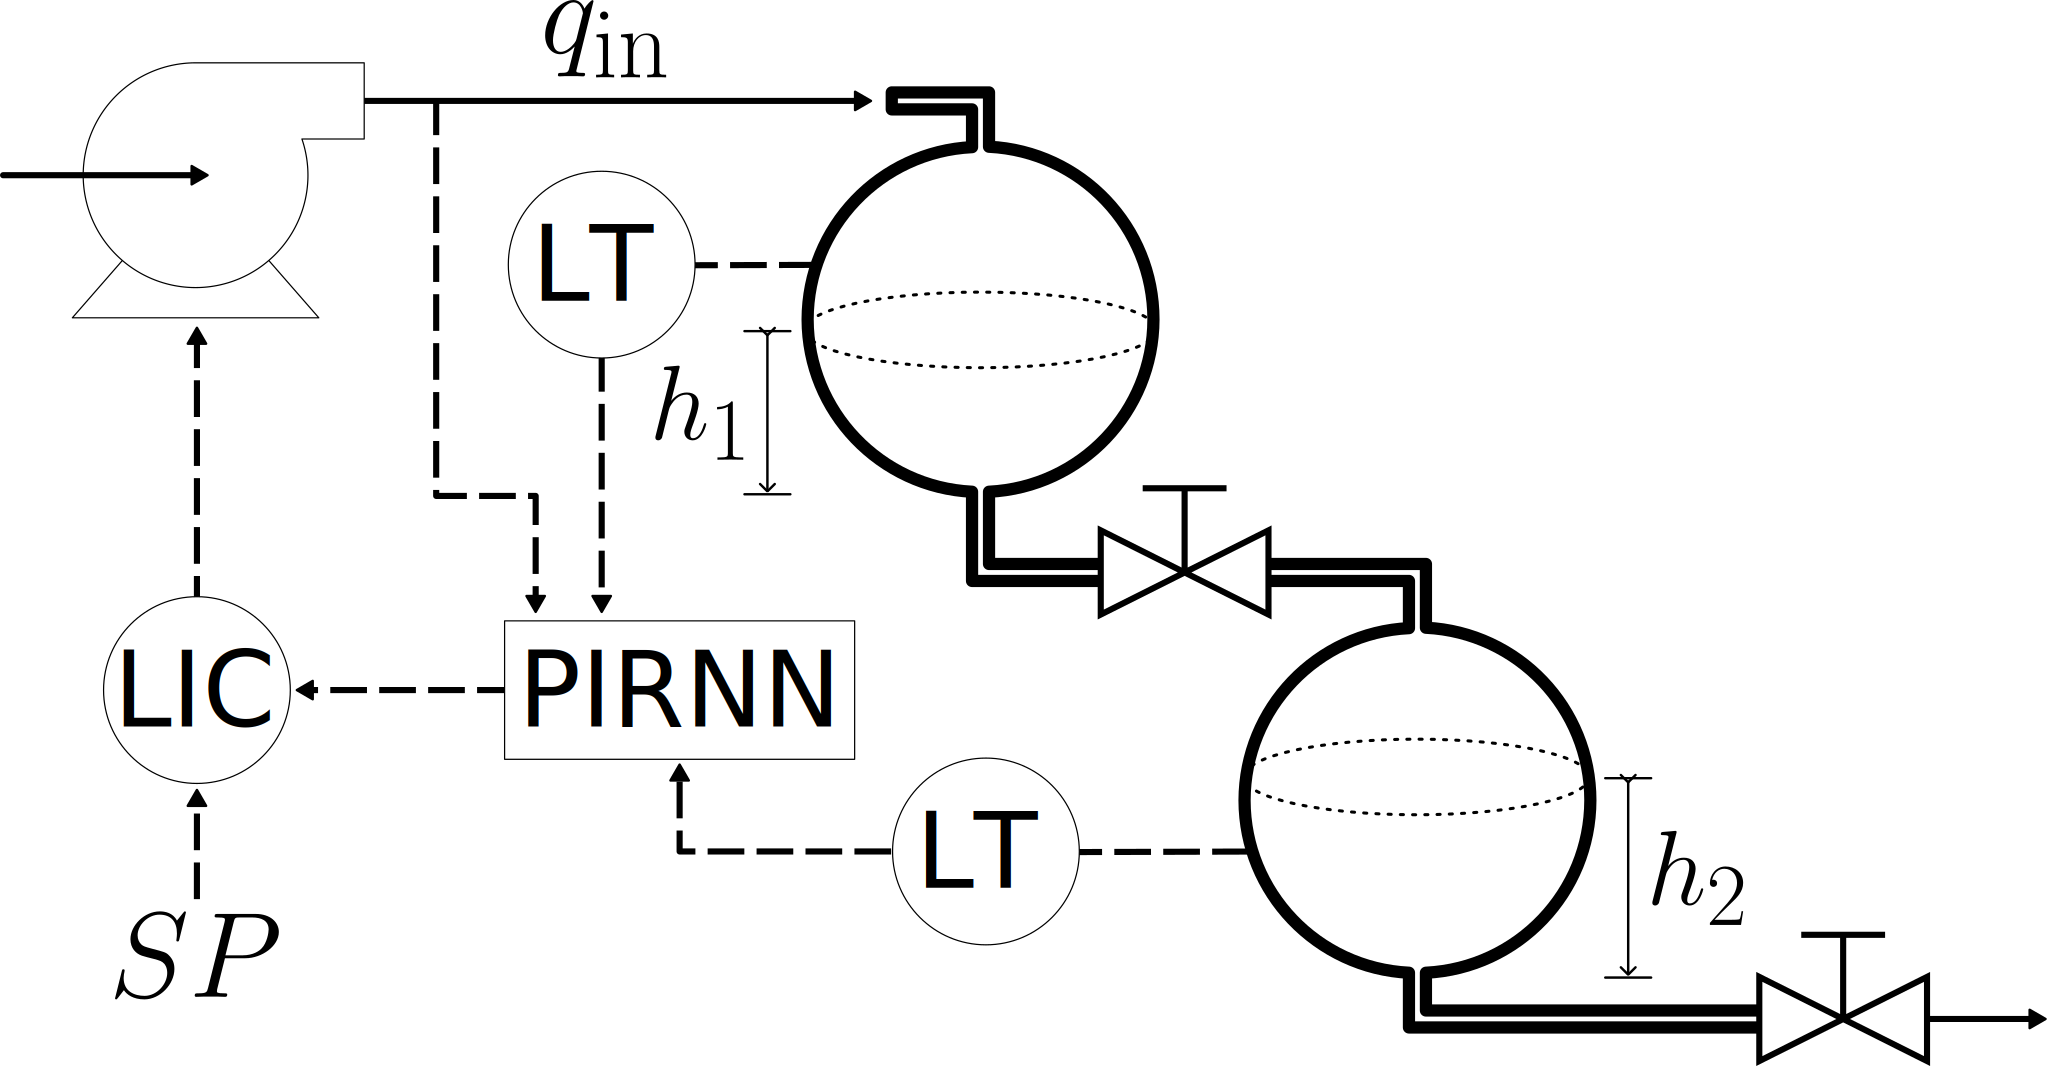
\includegraphics[width=\textwidth]{process-diagram/full.png}}
      \only<3>{\includegraphics[width=\textwidth]{process-diagram/feedback-1.png}}
      \only<4>{\includegraphics[width=\textwidth]{process-diagram/feedback-2.png}}
      \only<5>{\includegraphics[width=\textwidth]{process-diagram/feedback-3.png}}
      \caption{Representação esquemática do sistema.}
      \label{fig:tank-system}
    \end{figure}

    \column{0.5\textwidth}
    \begin{block}{Sistema de equações diferenciais dos tanques}
      \begin{subequations}
  \begin{align}
    \diff{h_1(t)}{t} & =
    \frac{
      q_{\mathrm{in}} - \alpha_1 s_1 \sqrt{2gh_1}
    }{
      \pi (2 R h_1 - h_1^2)
    }
    \label{eq:tank_system_a} \\[10pt]
    \diff{h_2(t)}{t} & =
    \frac{
      \alpha_1 s_1 \sqrt{2gh_1} - \alpha_2 s_2 \sqrt{2gh_2}
    }{
      \pi (2 R h_2 - h_2^2)
    }
    \label{eq:tank_system_b}
  \end{align}
\end{subequations}

      \vspace{0cm}
    \end{block}

  \end{columns}
\end{frame}

\begin{frame}
  \begin{table}[ht]
  \centering
  \caption{Constantes do sistema de equações~\ref{eq:tank_system}.}
  \label{tab:tanks_params}
  \begin{tabular}{ccc}
    Símbolo    & Descrição                          & Valor               \\ \hline
    $\alpha_1$ & Fator de correção 1                & $0.56$              \\
    $\alpha_2$ & Fator de correção 2                & $0.30$              \\
    $s_1$      & Área da seção de saída do tanque 1 & $0.50 \, cm^2$      \\
    $s_2$      & Área da seção de saída do tanque 2 & $0.50 \, cm^2$      \\
    $g$        & Aceleração da gravidade            & $980.665 \, cm/s^2$ \\
    $R$        & Raio dos tanques                   & $14.85 \, cm$       \\ \hline
  \end{tabular}
\end{table}
\end{frame}

\section{Metodologia}

\subsection{Descrição do Sistema e Modelagem matemática}

O sistema utilizado neste trabalho, conforme descrito por \citet{wildson_2024}, é composto por dois tanques esféricos interligados, como mostrado na Figura \ref{fig:tank-system}. Ambos sujeitos à pressão atmosférica. A dinâmica do sistema inclui uma entrada de fluido para o tanque 1 e uma saída de fluido do tanque 2, cuja vazão depende diretamente do nível do líquido no segundo tanque. Para simplificar as equações, assume-se que o líquido é incompressível e possui massa específica constante.

\begin{figure}[ht]
  \centering
  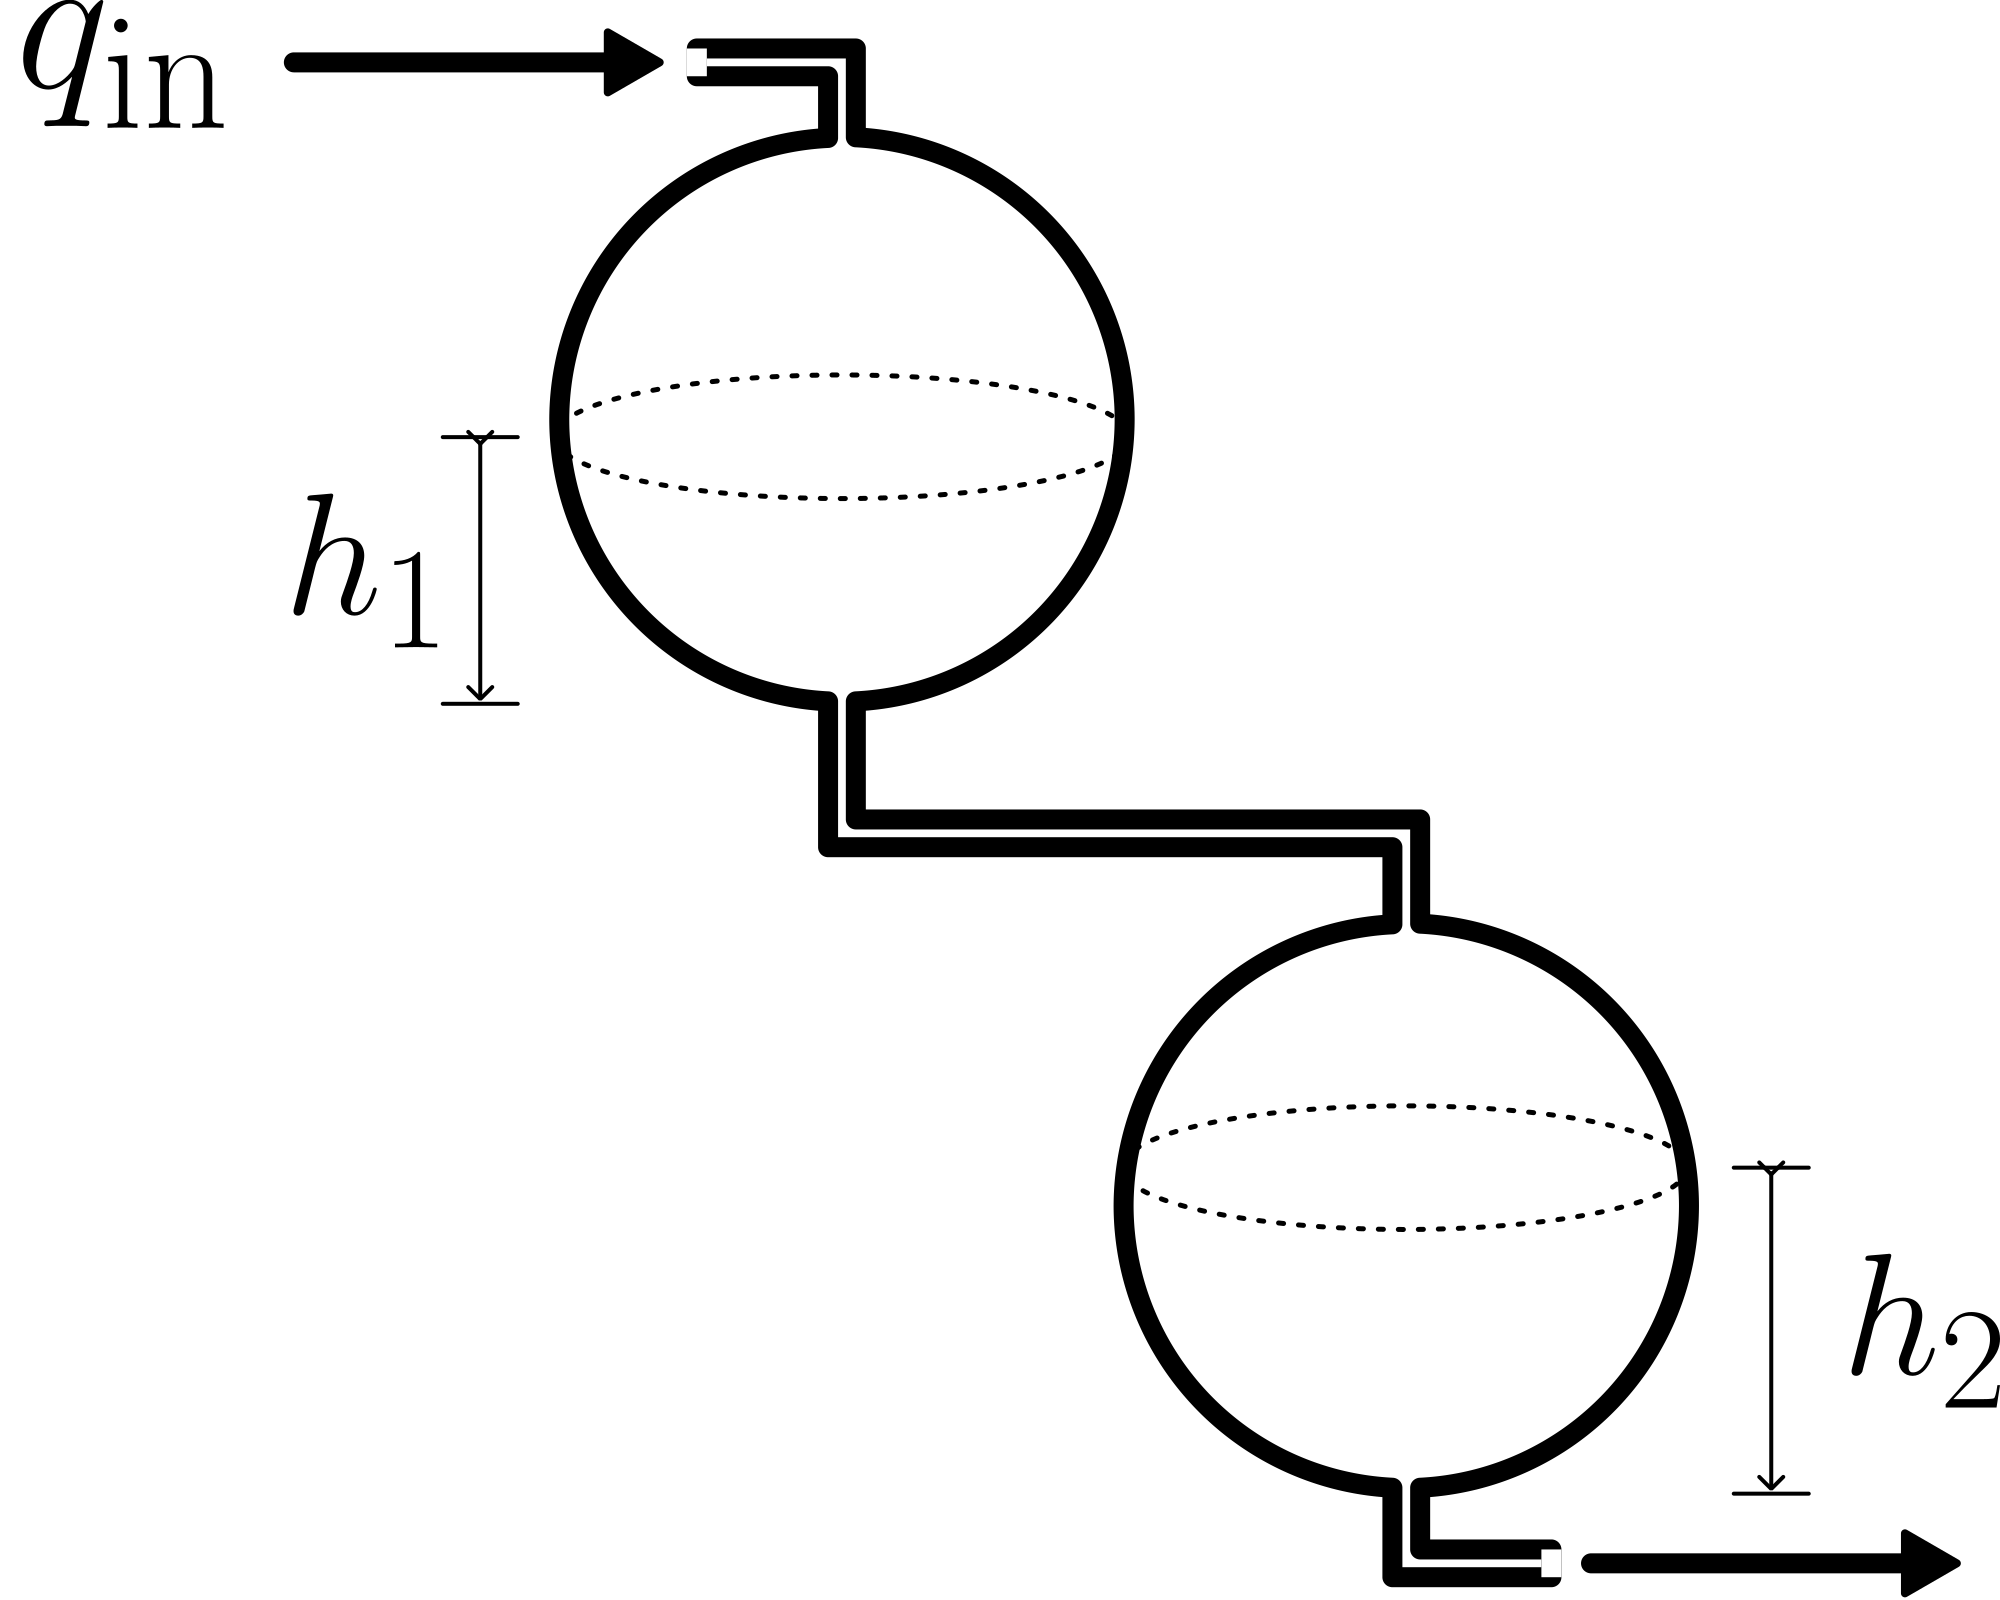
\includegraphics[width=0.3\textwidth]{tank-system.png}
  \caption{Representação esquemática do sistema de dois tanques esféricos.}
  \label{fig:tank-system}
\end{figure}

A modelagem baseia-se no princípio de conservação de massa, onde a taxa de variação do volume de líquido em cada tanque é dada pela diferença entre a vazão de entrada $q_{\mathrm{in}}$ e de saída $q_{\mathrm{out}}$, conforme a equação:
\begin{equation}
  \diff{V(t)}{t}=q_{\mathrm{in}}-q_{\mathrm{out}}
  \label{eq:conservation_of_mass}
\end{equation}

Para expressar a equação \ref{eq:conservation_of_mass} em termos de nível de líquido, é necessário dividir ambos os lados pela área da seção transversal do tanque, que, no caso de um tanque esférico, é uma função não linear da altura do líquido.

Como o sistema trata de dois tanques interligados, a vazão de saída do tanque 1 torna-se a vazão de entrada do tanque 2. Assim, a dinâmica de um tanque afeta diretamente o outro. Com isso, obtemos o sistema de equações diferenciais:

\begin{subequations}
  \begin{align}
    \diff{h_1(t)}{t} & =
    \frac{
      q_{\mathrm{in}} - \alpha_1 s_1 \sqrt{2gh_1}
    }{
      \pi (2 R h_1 - h_1^2)
    }
    \label{eq:tank_system_a} \\[10pt]
    \diff{h_2(t)}{t} & =
    \frac{
      \alpha_1 s_1 \sqrt{2gh_1} - \alpha_2 s_2 \sqrt{2gh_2}
    }{
      \pi (2 R h_2 - h_2^2)
    }
    \label{eq:tank_system_b}
  \end{align}
\end{subequations}
%
que descrevem a variação temporal do nível de líquido em cada tanque.

O valor e o significado de cada um dos parâmetros e constantes utilizados na modelagem, como área da seção transversal da tubulação e coeficientes relacionados à geometria dos tanques, são descritos com seus valores na Tabela \ref{tab:tanks_params}.

\begin{table}[ht]
  \centering
  \caption{Constantes do sistema de equações~\ref{eq:tank_system}.}
  \label{tab:tanks_params}
  \begin{tabular}{ccc}
    Símbolo    & Descrição                          & Valor               \\ \hline
    $\alpha_1$ & Fator de correção 1                & $0.56$              \\
    $\alpha_2$ & Fator de correção 2                & $0.30$              \\
    $s_1$      & Área da seção de saída do tanque 1 & $0.50 \, cm^2$      \\
    $s_2$      & Área da seção de saída do tanque 2 & $0.50 \, cm^2$      \\
    $g$        & Aceleração da gravidade            & $980.665 \, cm/s^2$ \\
    $R$        & Raio dos tanques                   & $14.85 \, cm$       \\ \hline
  \end{tabular}
\end{table}

\subsection{Desenvolvimento e Estrutura da Rede Neural}

As ANNs são modelos computacionais inspirados no funcionamento do cérebro humano. Elas consistem em camadas compostas de neurônios artificiais, elementos de processamento capazes de receber entradas e produzir uma saída com base em funções matemáticas. Cada neurônio realiza operações simples sobre suas entradas e as transmite para os neurônios da camada seguinte, permitindo a construção de representações mais complexas à medida que os dados passam pelas camadas da rede neural \citep{mu_sun_2022}. Elas são amplamente utilizadas na indústria química por sua capacidade de processar dados complexos e não-lineares comuns a essa indústria, tudo isso sendo consideradas modelos do tipo ``caixa preta'', onde as relações matemáticas entre variáveis não precisam ser conhecidas de antemão. Isso é especialmente útil quando não se tem um bom modelo matemático para o sistema, por ser possível construir modelos baseados unicamente em dados \citep{wang_2022}.

Entretanto, os modelos puramente baseados em dados apresentam limitações consideráveis. Para que esses modelos sejam eficazes, eles demandam um grande volume de dados representativos e abrangentes, algo nem sempre viável. Além disso, eles carecem de capacidade para extrapolar além das condições observadas nos dados de treinamento. Outro ponto crítico é que esses modelos podem gerar previsões inconsistentes com o conhecimento científico existente, pois não consideram as leis físicas que governam o sistema \citep{karniadakis_2021}. Então, para superar essas limitações e aproveitar o conhecimento físico disponível, surgiram as PINNs, introduzidas por \citeauthor{raissi_2017_I} em \citeyear{raissi_2017_I}. Elas Funcionam de forma parecida com às redes neurais artificiais tradicionais, com a diferença de que, além do custo associado aos dados, a função de custo também considera o erro relacionado ao problema físico, ou seja, a rede neural é penalizada ao diferir das relações físicas já conhecidas.

Da mesma maneira, as PIRNNs foram propostas como uma extensão das PINNs, combinando sua capacidade de incorporar conhecimento físico com a habilidade das redes neurais recorrentes (\textit{Recurrent Neural Networks} — RNNs) de processar dados sequenciais e capturar dependências temporais eficientemente \citep{zheng_2023}.

No caso da PIRNN utilizada neste trabalho, as entradas são compostas por dois valores anteriores dos estados do sistema ($h_1$, $h_2$) e da vazão de entrada $q_{\mathrm{in}}$, enquanto a saída da rede corresponde aos próximos valores dos níveis dos tanques. Dependendo da aplicação, a entrada pode ser composta por um valor anterior e um atual ($t{-}1$ e $t$) para a rede retornar o valor futuro ($t{+}1$), ou, como foi utilizado neste trabalho, dois pontos anteriores ($t{-}2$ e $t{-}1$) para retornar o valor presente ($t$). A arquitetura da rede é composta por uma camada recorrente do tipo \textit{Elman} \citep{elman_1990} seguida por camadas lineares totalmente conectadas. Para treiná-la, a função de custo adotada é composta pela soma do custo associado as equações diferenciais ($L_{\mathrm{EDOs}}$) e o custo relacionado aos dados de treinamento ($L_{\mathrm{data}}$). Os dados utilizados foram obtidos por meio de simulações computacionais com métodos numéricos tradicionais, uma vez que a física do problema está bem definida e permite gerar dados confiáveis para a modelagem. No total, a função de custo é definida como:
\begin{equation}
  L = \omega_1 \cdot L_{\mathrm{EDOs}} + \omega_2 \cdot L_{\mathrm{data}},
\end{equation}
onde
\begin{equation}
  \begin{aligned}
    L_{\mathrm{EDOs}} & = \frac{1}{N} \sum_{i=1}^{N} ( \diff{y_{\mathrm{prev},i}}{t} - f(y_{\mathrm{prev},i}))^2 \\
    L_{\mathrm{data}} & = \frac{1}{N} \sum_{i=1}^{N} (y_{\mathrm{data},i} - y_{\mathrm{prev},i})^2
  \end{aligned}
\end{equation}
Sendo os pesos $\omega_1$ e $\omega_2$ coeficientes ajustáveis que determinam a importância relativa de cada termo na função de custo, $y_{\mathrm{data}}$ os dados obtidos pela simulação, $y_{\mathrm{prev}}$ os valores de saída previstos pela rede neural e $f$ o sistema de equações diferencias \ref{eq:tank_system}. A derivada em relação ao tempo foi calculada por meio do método das diferenças finitas com 3 pontos, considerando os dois pontos fornecidos para a rede e o ponto previsto pela rede.

O treinamento da rede foi realizado utilizando o otimizador \textit{Adam} no framework PyTorch \citep{kingma_2017, pytorch_2024}. Para otimizar a inferência em tempo de execução, o modelo treinado foi convertido para o formato ONNX (\textit{Open Neural Network Exchange}), e os testes de velocidade foram realizados com o framework \textit{ONNX Runtime} \citep{onnxruntime}.

\subsection{Implementação no Arduino}

Criado em 2005, o Arduino é uma plataforma prototipagem amplamente utilizada por programadores devido ao seu baixo custo e facilidade para desenvolver. A plataforma conta com uma série de placas diferentes, cada uma com características específicas, para atender a diversas necessidades e aplicações. Entre as placas mais populares, destaca-se o Arduino UNO, uma das primeiras e mais acessíveis opções disponíveis e que foi a escolhida para esse trabalho \citep{hughes_2016}.

No entanto, o Arduino é bem limitado em termos de capacidade de memória e processamento. O modelo UNO, possui 32 kilobytes de memória flash e apenas 2 kilobytes de memória RAM, o que dificulta bastante a tarefa de implementar algoritmos mais complexos, como redes neurais que possuem muitas camadas. Nesse trabalho, para garantir que o código fosse compatível com as restrições do hardware, foram feitas otimizações para reduzir o uso de memória e armazenamento. Dentre elas, vale a pena destacar o uso da memória flash para armazenamento dos pesos e bias da rede neural por meio da diretiva \textit{PROGMEM} \citep{margolis_2020}. Isso é possível, pois esses valores são constantes, uma vez que foram definidos na etapa de treinamento da rede.

% Pequena gambiarra aqui. Essas duas figuras tiveram que mudar de posição para ajuste de layout.
\begin{figure}[ht]
  \centering
  \includegraphics[width=0.4\textwidth]{tanksim.png}
  \caption{Captura de tela do TankSim.}
  \label{fig:interface}
\end{figure}

\begin{figure*}[ht]
  \centering
  \includegraphics[width=0.8\textwidth]{sil-pirnn.png}
  \caption{Comparação entre as leituras dos sensores, obtidas a partir dos níveis simulados com adição de ruído, e os níveis previstos pela PIRNN embarcada após uma perturbação do tipo degrau na vazão de entrada. A linha tracejada vermelha vertical indica o instante em que os valores dos sensores deixam de ser enviados ao Arduino, fazendo com que a PIRNN passe a se retroalimentar.}
  \label{fig:sil-pirnn}
\end{figure*}

Para realizar a comunicação com o Arduíno, foi desenvolvido o \textit{software} \textit{TankSim} (Figura \ref{fig:interface}), responsável por simular o funcionamento do sistema, enviar os dados simulados para o Arduino e receber os valores previstos pela rede neural, além de plotar os gráficos comparando os dados simulados com os previstos. A interface conta ainda com um controle deslizante que permite o usuário alterar a vazão de entrada $q_{\mathrm{in}}$, dois interruptores para suspender o envio dos dados simulados do nível dos tanques para o Arduino e outro controle deslizante para controlar o nível de ruído. A interface foi programada utilizando o framework \texttt{Qt} (\url{https://www.qt.io/}), que oferece uma ampla gama de componentes e ferramentas para a criação de interfaces.

%alterar os valores de $\alpha_1$ e $\alpha_2$ (visando simular a degradação do modelo frente a uma mudança nos parâmetros dos tanques)

% Local original da figura fig:interface

No total, este sistema configura-se como um esquema \textit{software-in-the-loop} (SIL) \citep{chen_2008}. Nele, o \textit{TankSim} simula o envio de dados dos sensores de uma planta para o Arduino, que, por sua vez, responde com os dados previstos pela rede neural, ou seja, os prováveis valores para o nível de líquido em cada tanque no próximo intervalo de tempo. Quando os dados dos sensores não estão disponíveis, simulando uma falha ou interrupção manual por meio dos interruptores da interface, o Arduino entra em um modo de retroalimentação. Nesse modo, ele utiliza os valores previstos pela rede neural como entrada para gerar a previsão do próximo valor, mantendo a operação do sistema mesmo com os sensores indisponíveis.

\section{Resultados e Discussão}

Os resultados obtidos demonstram ser possível embarcar PIRNNs em plataformas de baixo custo com eficiência e robustez. Essa compatibilidade torna essa abordagem particularmente atrativa para aplicações industriais e acadêmicas que possuem restrições orçamentárias, permitindo a implementação de soluções de controle e simulação em larga escala sem a necessidade de hardware especializado ou de alto custo. Outro fator positivo foi o espaço ocupado pelo programa: verificou-se que o programa completo, que inclui tanto o modelo quanto o código responsável pela comunicação serial com o computador, utilizou apenas 68,4\% da memória flash e 13,2\% da memória RAM do Arduino. Esses números indicam que existem recursos disponíveis para implementação de modelos mais complexos ou execução de tarefas adicionais, caso necessário.

Nos testes de robustez, foram simulados cenários com ruído nas medições e com ausência completa de medições. A Figura \ref{fig:sil-pirnn} apresenta os resultados obtidos nesses testes. Observa-se que, no caso de medições ruidosas, o modelo capta as variações impostas pelo ruído, mas com um leve amortecimento, sugerindo uma capacidade de filtragem parcial das perturbações. Quando as medições são interrompidas completamente, o modelo passa a se retroalimentar. Nesse cenário, o modelo continua seguindo com precisão o comportamento esperado dos tanques, mesmo sem a entrada de dados dos sensores.

% Local original da figura fig:sil-pirnn

Nos testes de desempenho, a PIRNN demonstrou uma significativa vantagem em termos de velocidade quando comparada com métodos numéricos tradicionais. A comparação foi feita com os métodos RK, CVODES e IDAS da biblioteca \textit{CasADi}, e os métodos RK45, RK23 e LSODA da biblioteca \textit{SciPy}, todos executados no mesmo computador. Para avaliar o desempenho de cada método, foram realizadas 100 medições do tempo necessário para simular aproximadamente 33 horas de operação, considerando intensas perturbações na vazão de entrada. A Figura \ref{fig:pirnn-benchmark-lite} apresenta o boxplot dos tempos de execução dos métodos avaliados, evidenciando a superioridade da PIRNN em termos de tempo de processamento.

\begin{figure}[ht]
  \centering
  \includegraphics[width=0.45\textwidth]{pirnn-boxplot.png}
  \caption{Boxplot dos tempos de execução em escala de logaritmo natural dos métodos avaliados.}
  \label{fig:pirnn-benchmark-lite}
\end{figure}

Esses resultados mostram que o uso de PIRNNs embarcadas pode ser uma alternativa viável aos métodos tradicionais na simulação e controle de sistemas. A arquitetura proposta mostrou-se capaz de fornecer respostas rapidamente, o que é essencial para aplicações de controle em tempo real. Além disso, os testes de robustez demonstraram que a PIRNN manteve a qualidade das previsões mesmo em cenários adversos, como a presença de ruídos ou ausência de medições.

\section{Considerações finais}

Neste trabalho, foi demonstrada a utilização de uma PIRNN embarcada em um Arduino UNO para simular um sistema dinâmico formado por dois tanques esféricos em cascata. Os resultados mostraram que a PIRNN é uma alternativa viável aos métodos numéricos tradicionais e apresenta desempenho superior em relação ao tempo de simulação, sem grandes prejuízos a fidelidade das previsões. Isso a torna adequada para o controle em tempo real, sendo aplicável em automação industrial, monitoramento de processos e como analisador virtual. Sua compatibilidade com plataformas de baixo custo, como o Arduino, torna-a acessível e robusta, mantendo boa desempenho mesmo com falhas ou ruídos nas medições.

Contudo, em sistemas dinâmicos reais, é necessário considerar a degradação dos parâmetros do modelo ao longo do tempo, causada pelo desgaste ou envelhecimento dos componentes físicos. Essa degradação pode comprometer o desempenho da PIRNN, tornando necessário o retreinamento periódico do modelo para garantir sua acurácia. Nesse contexto, estudos futuros podem explorar técnicas de aprendizado por reforço, visando a adaptação em tempo real da PIRNN às mudanças dos parâmetros do sistema sem a necessidade de intervenções manuais.

Por fim, pesquisas adicionais podem investigar a implementação de modelos mais complexos, visando expandir a aplicabilidade das PIRNNs em sistemas dinâmicos descritos por equações diferenciais parciais.


\section*{Agradecimentos}
Os autores gostariam de agradecer o suporte financeiro da ANP no âmbito do PRH 35.1.

\bibliography{../common/bibliography.bib}

\end{document}
